\documentclass{article}
\usepackage{fullpage}
\usepackage{parskip}
\usepackage{hyperref}
\usepackage{listings}
\usepackage{graphicx}
\usepackage[usenames,dvipsnames]{color}
\hypersetup{
    colorlinks,
    citecolor=Red,
    linkcolor=Red,
    urlcolor=Red}
\begin{document}

\title{Modern OpenGL Assignments Introduction and Setup}
\author{CS148 Fall 2015-2016}
\date{}
\maketitle

\textcolor{red}{WARNING: DO NOT COPY AND PASTE COMMANDS FROM THE PDF INTO THE TERMINAL. IT IS SAFER TO MANUALLY TYPE OUT THE COMMANDS YOURSELF.}

If you find any of the instructions below to be unclear, confusing, or otherwise incorrect please contact a CA or post on Piazza!

\section*{Requirements}

Note that the OpenGL assignments have been modernized to use OpenGL 4.1 and (the newest version supported by Mac OSX) as such it will be necessary to have updated compilers/operating systems/drivers. If for whatever reason you can not run the OpenGL 4.1 assignments, contact the CA's and we will get you setup with the old assignments (OpenGL 2).

You will need to make sure you have the following:
\begin{enumerate}
    \item C++ Compiler with C++11 Support
    \item OpenGL 4.1 Support
    \item CMake 2.8+
    \item Python 2.7.x
\end{enumerate}

If any of the instructions below are unclear, ask a CA or post on Piazza.

\subsection*{Windows}

\subsubsection*{C++ Compiler}

Download Visual Studio 2015 (Community Version) for FREE: \href{https://www.visualstudio.com/en-us/products/vs-2015-product-editions.aspx}{here} to make sure you have Microsoft's latest compiler.  Visual Studio 2013 should also work should you have that.

\subsubsection*{OpenGL 4.1 Support}

Your system should have the OpenGL headers already. Make sure your drivers are updated from Nvidia/AMD/Intel.

\subsubsection*{CMake}

Download the latest CMake binaries from the CMake website: \href{http://www.cmake.org/download/}{here}.

\subsubsection*{Python 2.7}

Download Python 2.7 from \href{https://www.python.org/download/releases/2.7/}{here}. Afterwards, make sure your PATH is set such that it the Python 2.7 binary directory included. If you have Python 3+ installed, make sure Python 3 is either not in the path or that running "python --version" in the command prompt runs Python 2.7 instead of Python 3.

\textcolor{red}{TODO: Insert pictures for setting the system path, Check to see what would happen if Python3 and Python2.7 both installed}.

\subsection*{Mac OSX}

\subsubsection*{C++ Compiler}

Make sure you have XCode installed. If you do not have XCode installed, you can go \href{https://developer.apple.com/xcode/download/}{here} to download it (it will redirect you to the app store). Make sure you download XCode 7 and not the XCode 7.1 beta. If you wish, you can click on 'Additional Tools' \href{https://developer.apple.com/downloads/}{(or here)} to find XCode 6.4.

\textcolor{red}{TODO: Test XCode 7}

\subsubsection*{OpenGL 4.1 Support}

Your system should have the OpenGL headers already once you install XCode. To see if your system supports OpenGL 4.1 look at Apple's OpenGL capabilities table: \href{https://developer.apple.com/opengl/capabilities/}{here}. To see what graphics card you have, you can click on the 'Apple' button and click on 'About this Mac' and in the window that pops up, your graphics card is displayed next to \textbf{Graphics}. Additionally, you'll want to make sure your Mac OS X is updated to at least 10.9 if not 10.10 (upgrade! It's free).

\textcolor{red}{TODO: Add pictures}

\subsubsection*{CMake}

Download the latest CMake binaries from the CMake website: \href{http://www.cmake.org/download/}{here}.

\subsubsection*{Python 2.7}

Download Python 2.7 from \href{https://www.python.org/download/releases/2.7/}{here} and install it. Running "python --version" in the terminal should display 2.7.x.

\subsection*{Linux}

Note that the instructions here are tailored to Ubuntu. If you have a different distribution, the steps should be similar as the only major difference should be the package names. Talk to a CA if you need help with this.

\subsubsection*{C++ Compiler}

On Linux, you'll want to be using G++ 4.6 or later. If possible, you'll want to be using G++ 4.8.1 or GCC 5+. On Ubuntu you can run:

\begin{lstlisting}
sudo apt-get install g++-4.8
\end{lstlisting}

You will also be needing to run the 'make' command so generally it is recommended that you install the 'build-essentials' package (on Ubuntu).

\begin{lstlisting}
sudo apt-get install build-essentials
\end{lstlisting}

The G++ 4.8 package is available on Ubuntu 14.04 LTS or later! If you have another distribution, check your distribution package mananager to see what version of G++ they have. If you have any problems with another distribution, contact a CA!

\subsubsection*{OpenGL 4.1 Support}

Make sure you have the latest drivers for your GPU. After you installed the drivers (be it open source or closed source), you can double check to make sure you have OpenGL 4.1 by installing the "mesa-utils" package on Ubuntu (may be named "mesa-demos" on other distributions). Then in the terminal run, 'glxinfo | grep "OpenGL version"' and make sure you get a version that's greater than or equal to 4.1!

\subsubsection*{CMake}

You can download the latest CMake using your package manager. On Ubuntu, you can run:

\begin{lstlisting}
sudo apt-get install cmake
\end{lstlisting}

\subsubsection*{Python 2.7}

In your command line, type "python --version" to see what version of Python you have/if it is installed. If it is not installed, or if you have the wrong version, you will want to run (on Ubuntu): 

\begin{lstlisting}
sudo apt-get install python
\end{lstlisting}

\section*{Compiling}

Compiling is a two step process regardless or whether you are using the CMake GUI or the CMake Command-Line Interface (CLI). First you will use CMake to generate the proper build files (Visual Studio, XCode, or Makefiles) and use Visual Studio/Xcode/Makefiles to actually build the application (aptly named cs148opengl4). This section assumes that you have the assignment code unzipped somewhere. 

\subsection*{CMake Configuration and Generation}

\subsubsection*{Special Notes for Visual Studio Solutions and XCode Projects}

If you are using CMake to generate for Visual Studio or XCode, you can run CMake once (the very first time) and then use Visual Studio or Xcode to manage any new files you might add (instead of using CMake to do that for you). However, should you ever run CMake again, you will overwrite your Visual Studio solution/XCode project and lose any changes you made. To avoid having to run CMake to compile a new assignment, you can instead go into "main.cpp" and after the include statements, add a line that says 
\begin{lstlisting}
#define ASSIGNMENT N
\end{lstlisting}

where N is the assignment you wish to compile for (1, 2, 3).

\subsubsection*{GUI (Windows, Mac OSX)}

The images below are for CMake 3.3 on Mac OS X but they should be relevant for Windows as well. Open CMake and point 'Where is the source code' to the 'source' folder located wherever you extracted the assignment framework and point 'Where to build the binaries' to 'build/xcode' if you are on Mac OSX or 'build/vs' if you are on Windows (though it doesn't really matter, you can make your own folder if you really wanted to...).

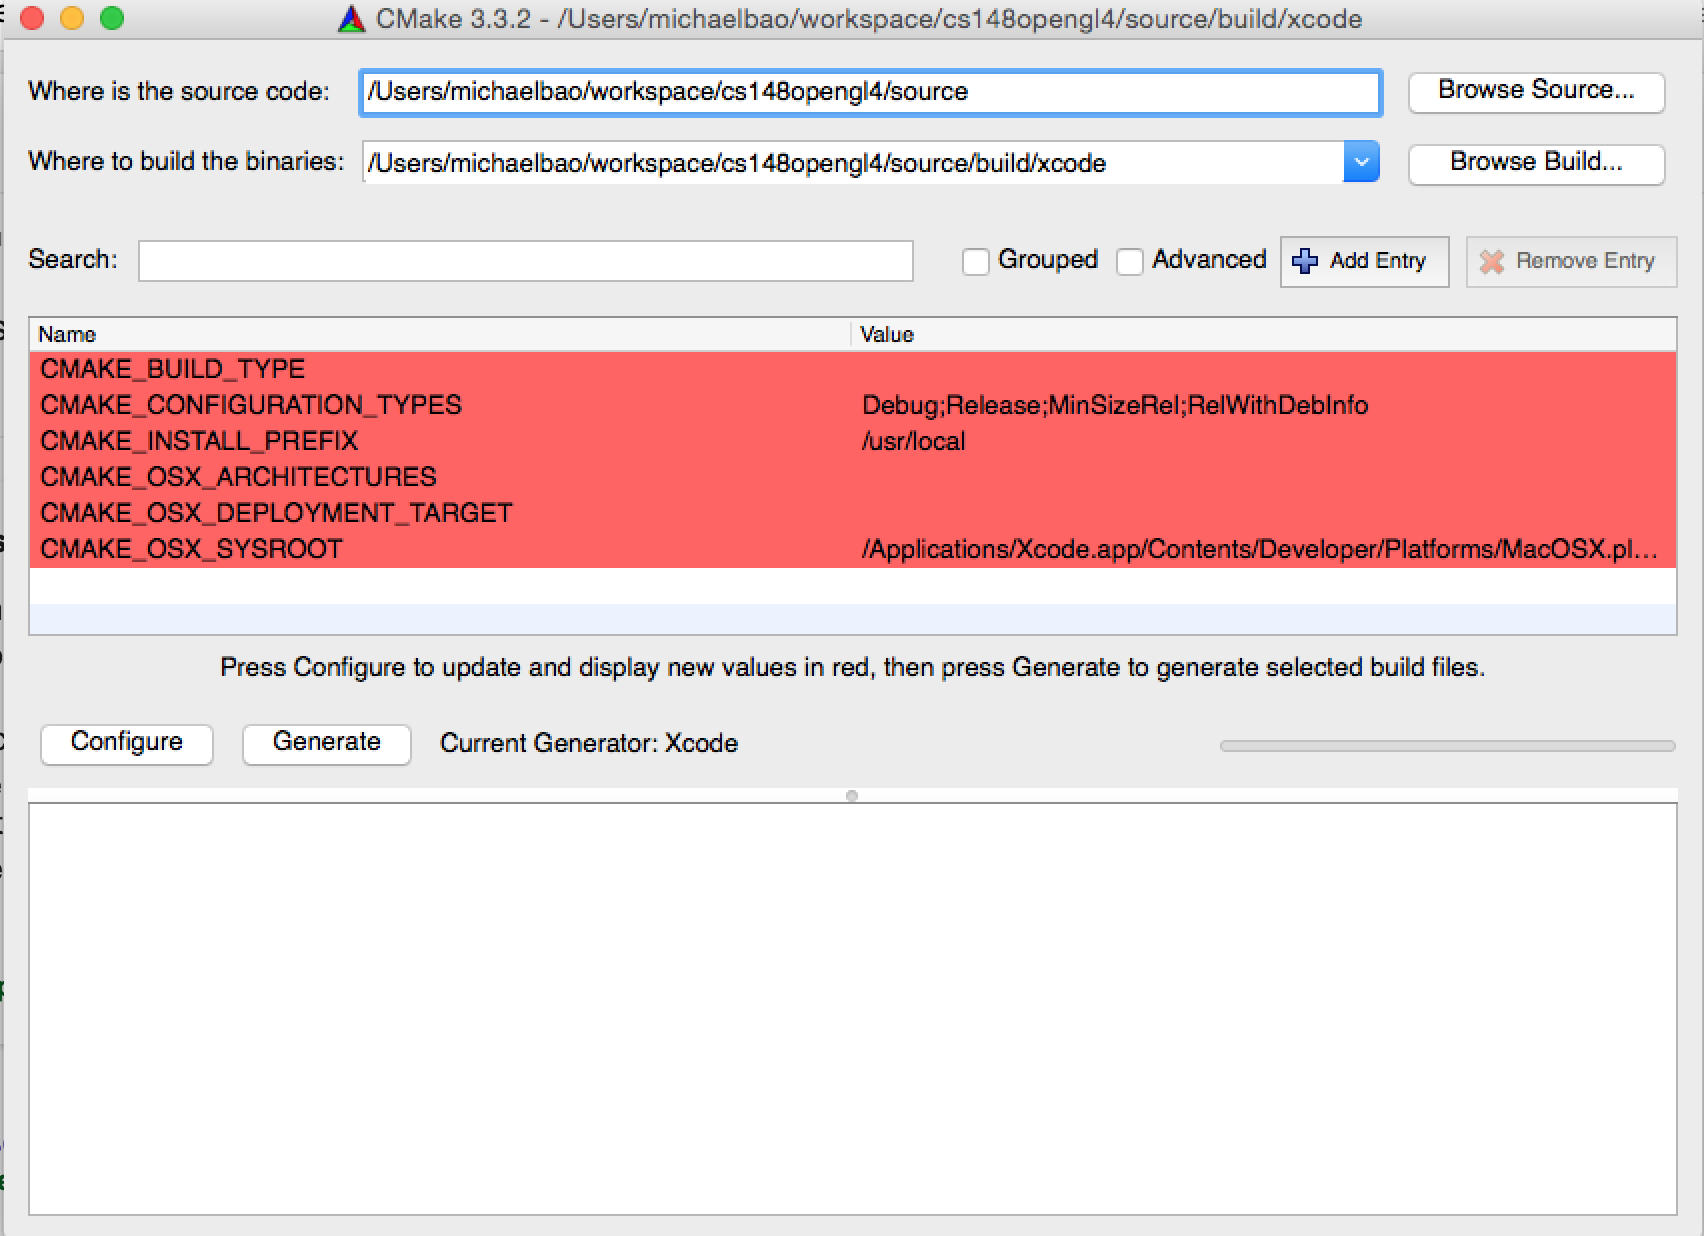
\includegraphics[width=\linewidth]{cmake1.png}

Afterwards, click the 'Add Entry' button with 'Name' set to "ASSIGNMENT", 'Type' set to 'STRING' and Value set to N where N is the assignment number that you wish to compile (1, 2, 3).

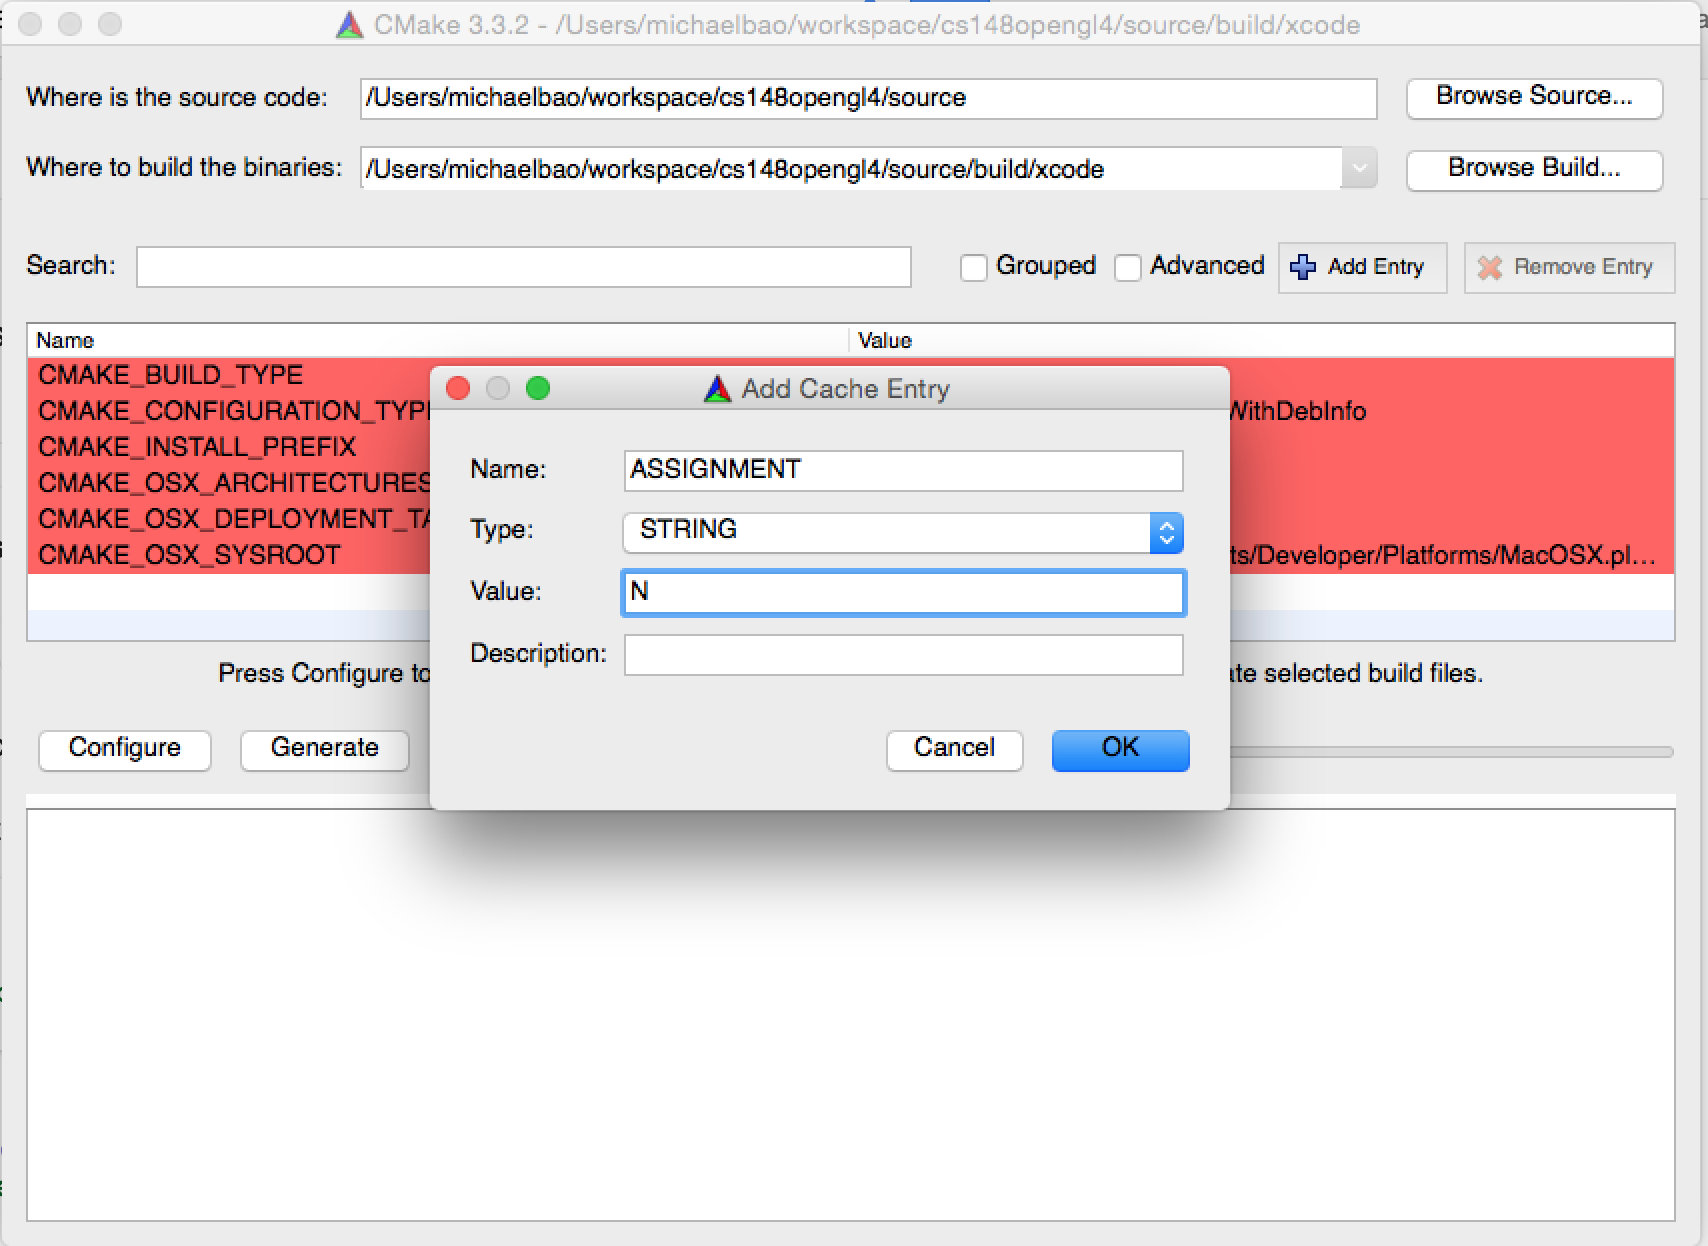
\includegraphics[width=\linewidth]{cmake2.png}

At this point, you can click the Configure button and then the Generate button. Now your Visual Studio solution or XCode project should exist within your previously selected build folder.

\subsubsection*{CLI (Linux, Mac OS X)}

Usually, you'll only be using the CLI on Mac or Linux so I will be ignoring Windows here. If you want to generate the build files for XCode, first go into the "build/xcode" directory and then run: 

\begin{lstlisting}
cmake ../../ -G "Xcode" -DASSIGNMENT=N
\end{lstlisting}

where N is the assignment you are trying to compile (1, 2, 3). Afterwards, the file "cs148-opengl4.xcodeproj" will exist and you will be able to open it up in XCode.

If you want to generate Makefiles, go into "build/unix" and then either go into the Release or Debug folder. Then you will want to run:

\begin{lstlisting}
cmake ../../../ -G "Unix Makefiles" -DASSIGNMENT=N -DCMAKE_BUILD_TYPE=CONFIG
\end{lstlisting}

In this case, N is the assignment you are trying to compile (1, 2, 3) and CONFIG is either Release or Debug depending on which folder you are in.

\subsection*{Compilation}

\subsubsection*{Visual Studio}

\textcolor{red}{TODO: WRITE INSTRUCTIONS HERE}

\subsubsection*{XCode}

In the upper left corner, your build target by default should be set to ALL\_BUILD, change it to cs148opengl4 (click on ALL\_BUILD).

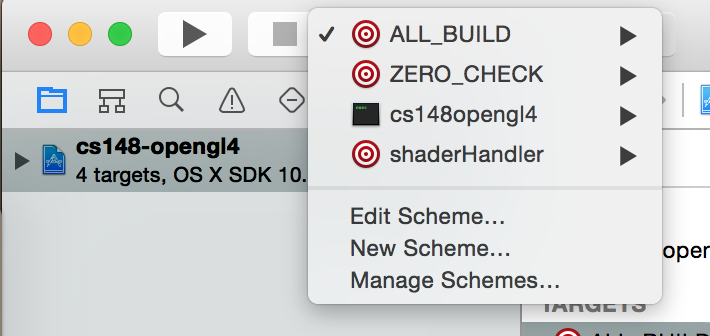
\includegraphics[]{xcode1.png}

At this point, you can hit the 'Play' button and it will compile and launch the application! However, if you ever want to change from a Debug build to a Relase build or vice versa, you will need to go same screen as before (click on cs148opengl4) and click on 'Edit Scheme...'. In the screen that pops up, make sure on the left, you have 'Run' selected and on the right, you are in the 'Info' tab. You should see a build configuration dropdown from which you can select the build type that you want.

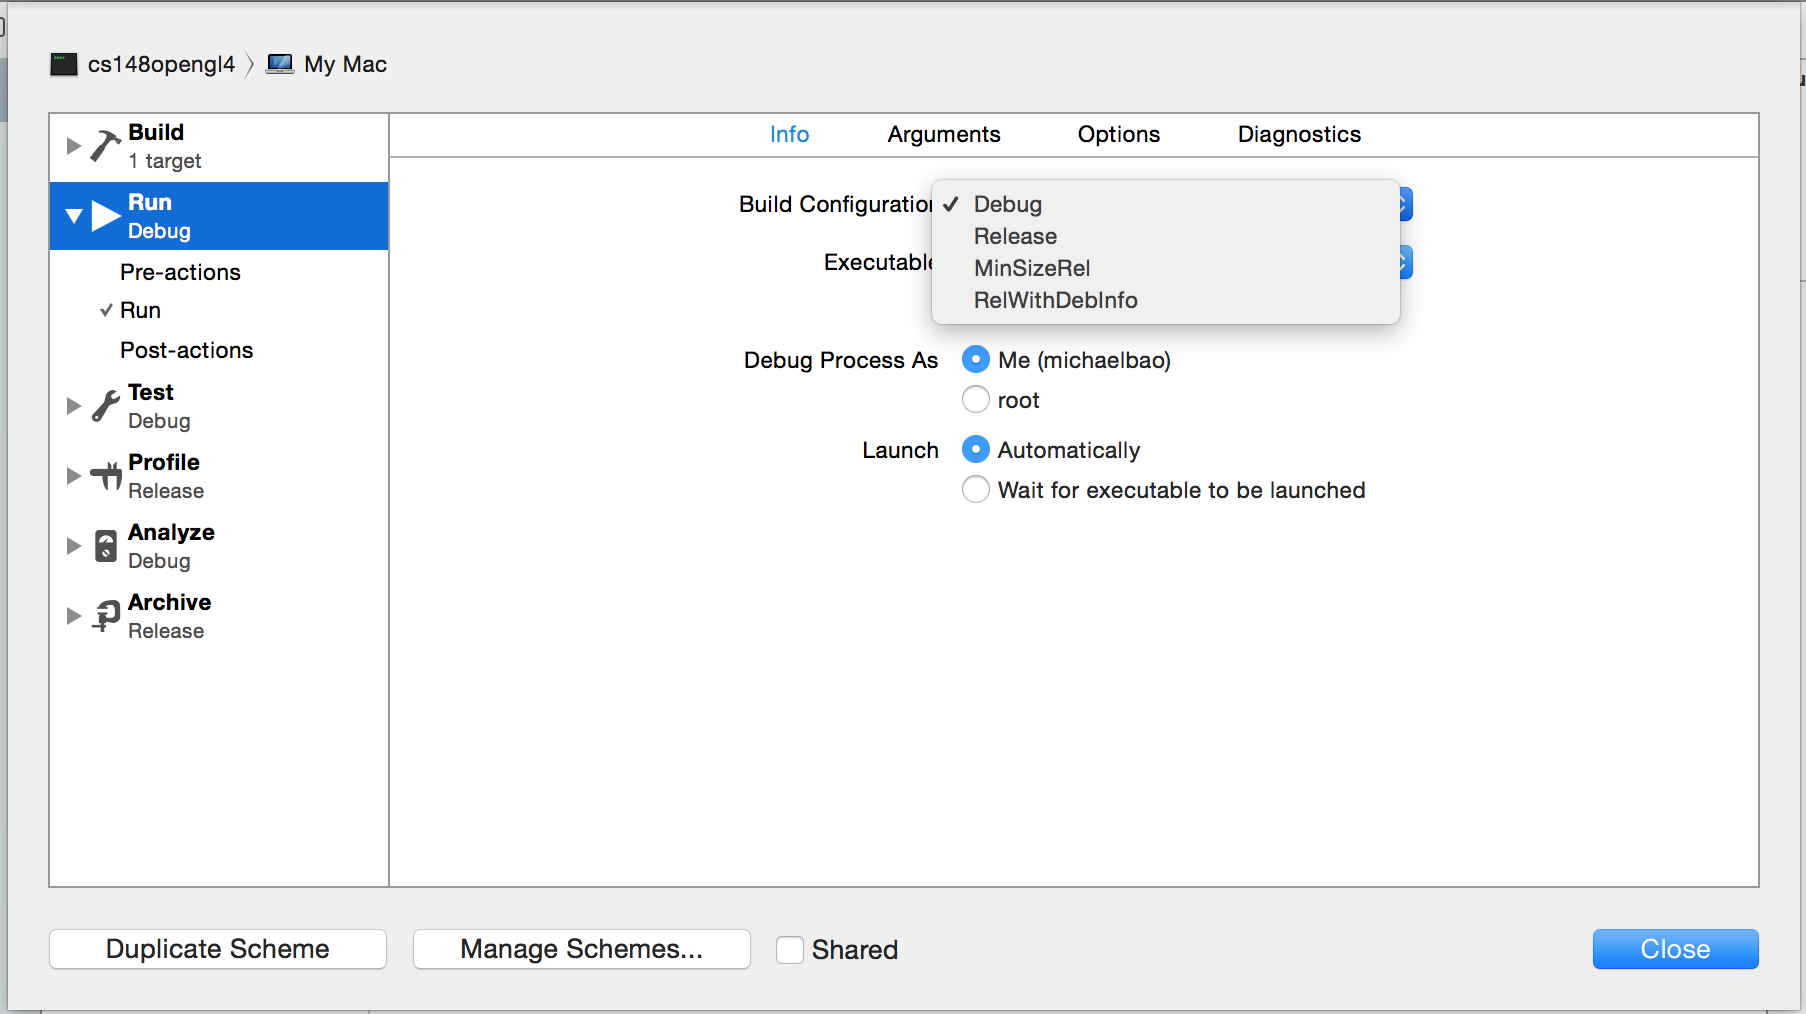
\includegraphics[width=\linewidth]{xcode2.png}

\subsubsection*{Makefiles}

Inside the build/unix/Debug or build/unix/Release folder, type

\begin{lstlisting}
make
\end{lstlisting}

or 

\begin{lstlisting}
make -jN
\end{lstlisting}

to use N cores (change N to 2 or 4, or however many cores you may have).

Afterwards, should compilation succeed, an executable named "cs148opengl4" will exist which you can run by typing 

\begin{lstlisting}
./cs148opengl4
\end{lstlisting}

\end{document}

